\section{Построение вольт-амперной характеристики нелинейного элемента на экране осциллографа}
\LabHeader{получить на экране вольт-амперную характеристику нелинейного элемента.}{источник переменного напряжения частотой, осциллограф, способный работать в режиме развертки по X от внешнего сигнала, нелинейный элемент (стабилитрон, диод и т.\,п.)}
{\itshape В данной работе требуется научиться работать с осциллографом}
\SolveVariant
\begin{wrapfigure}{o}{5.71cm}
	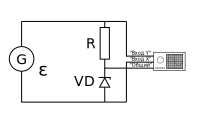
\includegraphics{11klOSC-1.pdf}
    \caption{Схема установки}
    \label{fig:11kl-vah-osc:scheme}
\end{wrapfigure}
Соберем схему, изображенную на рис.~\ref{fig:11kl-vah-osc:scheme}. Принцип работы установки следующий: за счёт подключенного через резистор генератора, на нелинейном элементе возникает переменное напряжение \(U(t)\), при этом через него течёт переменный ток \(I(t)\). В любой момент времени \(t_0\) точка \( \left( I(t_0); U(t_0) \right)\) лехит на кривой ВАХ данного нелинейного элемента. На <<Вход X>> поступает напряжение с нелинейного элемента, а на <<Вход Y>> "--- напряжение с добавочного сопротивления \(R\), пропорциональное току на нелинейном элементе. В силу особенностей устройства осциллографа на пластины, отклоняющие луч по X подаётся напряжение <<Вход X>>--<<Общий>>, а на отклоняющие по Y "--- <<Вход Y>>--<<Общий>>, изображение ВАХ на экране будет перевернутым относительно горизонтальной оси.\par
После того, как на экране осциллографа будет получена устойчивая картина, её следует перерисовать на бумагу вместе с координатной сеткой, отмасштабировать и нанести ось с учётом пересчёта напряжения на сопротивлении в ток через нелинейный элемент (\(I = \frac{U}{R}\)).
\MesErrors
Расчет в привычном смысле производить не нужно.
\SchoolBase
\begin{itemize}
    \item Вольт-амперная характеристика
    \item Идеальный диод
\end{itemize}
\AdditionalQuestions
\begin{itemize}
    \item Выполняется ли закон Ома для нелинейных элементов? Какие границы применимости закона Ома?\par
    \Answer В классической форме закон Ома применим лишь для простых материалов в ограниченном диапазоне токов и напряжений. Для нелинейных элементов можно говорить о сопротивлении, зависящем от напряжения на элементе. Также часто используется понятие <<дифференциальное сопротивление>>: $r(U) = \lim _ {\Delta U, \Delta I \rightarrow 0}\frac{\Delta U}{\Delta I}$
\end{itemize}
